% Emerald Publishing - Construction Innovation Submission Template
% by Oleksandr Melnyk
% Ver 0.0.4
% Based on: https://www.emeraldgrouppublishing.com/journal/ci#author-guidelines

\documentclass{article}

\usepackage[english]{babel}

% Set page size and margins
% Replace `letterpaper' with `a4paper' for UK/EU standard size
\usepackage[a4paper,top=2cm,bottom=2cm,left=3cm,right=3cm,marginparwidth=1.75cm]{geometry}

% Useful packages
\usepackage{amssymb}
\usepackage{amsmath}
\usepackage{siunitx}
\PassOptionsToPackage{hyphens}{url}\usepackage{hyperref}
\usepackage{cleveref}
\usepackage[utf8]{inputenc}
\usepackage[right]{lineno}
\usepackage{csquotes}
\usepackage{booktabs}
\usepackage{longtable}
\usepackage{adjustbox}
\usepackage{graphicx}
\usepackage{array}
\usepackage{url}
\usepackage{titlesec}
%\usepackage[compatibility=false]{caption}
\usepackage{authblk}
\usepackage{xcolor} % Load the xcolor package for color options
\usepackage{listings}
\usepackage{makecell}
\usepackage{subcaption}

\renewcommand{\thetable}{\Roman{table}}

% Define a new format for \subsection
\titleformat{\subsection}
  {\mdseries\itshape\large} % Medium series, italic shape, and large font size
  {\thesubsection}{1em}{} % Numbering, spacing, and the section title itself


% Emerald Harvard Citation Style

\usepackage[english]{babel}
\usepackage[style=authoryear,backend=biber,natbib=true,maxcitenames=2,uniquelist=false]{biblatex}
\addbibresource{bibliography.bib} % your .bib file

% Customizing biblatex for Harvard style
\DeclareNameAlias{sortname}{family-given}
\DeclareNameAlias{default}{family-given}

\renewbibmacro{in:}{}
\DeclareFieldFormat[article]{title}{\mkbibquote{#1}\addcomma}
\DeclareFieldFormat[book]{title}{\mkbibemph{#1}\addcomma}
\DeclareFieldFormat[bookinbook]{title}{\mkbibemph{#1}\addcomma}
\DeclareFieldFormat[inbook]{title}{\mkbibquote{#1}\addcomma}
\DeclareFieldFormat[incollection]{title}{\mkbibquote{#1}\addcomma}
\DeclareFieldFormat[inproceedings]{title}{\mkbibquote{#1}\addcomma}
\DeclareFieldFormat[manual]{title}{\mkbibemph{#1}\addcomma}
\DeclareFieldFormat[misc]{title}{\mkbibemph{#1}\addcomma}
\DeclareFieldFormat[thesis]{title}{\mkbibemph{#1}\addcomma}
\DeclareFieldFormat[unpublished]{title}{\mkbibquote{#1}\addcomma}
\DeclareFieldFormat[patent]{title}{\mkbibemph{#1}\addcomma}
\DeclareFieldFormat[report]{title}{\mkbibemph{#1}\addcomma}
\DeclareFieldFormat[online]{title}{\mkbibquote{#1}\addcomma}
\DeclareFieldFormat[software]{title}{\mkbibemph{#1}\addcomma}
\DeclareFieldFormat[booklet]{title}{\mkbibemph{#1}\addcomma}
\DeclareFieldFormat[periodical]{title}{\mkbibemph{#1}\addcomma}
\DeclareFieldFormat[standard]{title}{\mkbibemph{#1}\addcomma}

\DeclareFieldFormat[article]{journaltitle}{\iffieldundef{shortjournal}{\mkbibemph{#1}\addcomma}{\mkbibemph{\printfield{shortjournal}}\addcomma}}
\DeclareFieldFormat{volume}{\bibstring{volume}~#1}
\DeclareFieldFormat{number}{\bibstring{number}~#1}

% Definitions for "Vol." and "No."
\DefineBibliographyStrings{english}{
  volume = {Vol.},
  number = {No.}
}

\renewbibmacro*{volume+number+eid}{%
  \printfield{volume}%
  \setunit*{\addspace}%
  \printfield{number}%
  \setunit{\addcomma\space}%
  \printfield{eid}}

\renewbibmacro*{journal+issuetitle}{%
  \usebibmacro{journal}%
  \setunit*{\addcomma\space}%
  \usebibmacro{volume+number+eid}%
  \setunit{\addcomma\space}%
  \usebibmacro{issue+date}}

\renewbibmacro*{publisher+location+date}{%
  \printlist{publisher}%
  \iflistundef{location}
    {\setunit*{\addcomma\space}}
    {\setunit*{\addcolon\space}}%
  \printlist{location}%
  \setunit*{\addcomma\space}%
  \usebibmacro{date}}

\renewcommand*{\bibpagespunct}{\addcomma\space}

% Customizing page field format to prevent duplication
% \DeclareFieldFormat{pages}{%
%   \mkfirstpage[{\mkpageprefix[page]{#1}}]{#1}}

% Customizing citations for Harvard style
\DeclareCiteCommand{\cite}[\mkbibparens]
  {\usebibmacro{prenote}}
  {\usebibmacro{citeindex}%
   \usebibmacro{cite}}
  {\multicitedelim}
  {\usebibmacro{postnote}}

\renewbibmacro*{cite:labelyear+extrayear}{%
  \iffieldundef{labelyear}
    {}
    {\printtext[bibhyperref]{%
       \printfield{labelyear}%
       \printfield{extrayear}}}}

\renewbibmacro*{cite:labeldate+extradate}{%
  \iffieldundef{labelyear}
    {}
    {\printtext[bibhyperref]{%
       \printfield{labelyear}%
       \printfield{extradate}}}}

\AtEveryBibitem{
  \clearfield{month}
  \clearfield{day}
  \ifentrytype{book}{
    \clearlist{location}
  }{}
}

% Formatting "et al." in italics followed by a comma
\DefineBibliographyStrings{english}{
  andothers = {\textit{et al.},}
}

\DeclareFieldFormat[article]{volume}{\bibstring{jourvol}\addnbspace #1}
\DeclareFieldFormat[article]{number}{\bibstring{number}\addnbspace #1}
\DeclareFieldFormat[article]{volume}{Vol. #1}
\DeclareFieldFormat[article]{number}{No. #1}
% Customizing DOI field format to lowercase "doi"
%\DeclareFieldFormat{doi}{\bibstring{doi}\addcolon\space\url{#1}}

% Customizing URL field format to "available at:"
\DeclareFieldFormat{url}{\bibstring{available at}\addcolon\space\url{#1}}
\DeclareFieldFormat{urldate}{\mkbibparens{accessed \addspace#1}}

% Customizing urldate to match the required format
\DeclareFieldFormat{urldate}{%
  \mkbibparens{accessed\space%
    \thefield{urlday}\addspace%
    \mkbibmonth{\thefield{urlmonth}}\addspace%
    \thefield{urlyear}}}

% Configure cleveref
\crefformat{figure}{#2Figure~#1#3}
\Crefformat{figure}{#2Figure~#1#3}
\crefformat{table}{#2Table~#1#3}
\Crefformat{table}{#2Table~#1#3}
\crefformat{section}{#2Section~#1#3}
\Crefformat{section}{#2Section~#1#3}

%%% Flags, colors and comments
\definecolor{dkred}{rgb}{.6,0,0}
\definecolor{dkgreen}{rgb}{0,.5,0}
\newif\ifdraft\drafttrue
\newcommand{\displaycomment}[1]{{#1}} % inline
\newcommand\hl[1]{{\color{dkred} #1}}
\newcommand{\alt}{\uparrow}
\newcommand{\olremark}[2]{{\color{dkgreen}(#1: #2)}}
\newcommand{\varemark}[2]{{\color{dkred}(#1: #2)}}
\newcommand{\ftremark}[2]{{\color{teal}(#1: #2)}}
\newcommand{\pfremark}[2]{{\color{blue}(#1: #2)}}
\newcommand{\fsremark}[2]{{\color{violet}(#1: #2)}}
\newcommand{\acremark}[2]{{\color{purple}(#1: #2)}}
\newcommand{\lnegremark}[2]{{\color{cyan}(#1: #2)}}
\newcommand{\loliremark}[2]{{\color{orange}(#1: #2)}}
\ifdraft
\newcommand{\mmerenda}[1]{\varemark{MM}{#1}}
\newcommand{\scolli}[1]{\olremark{SC}{#1}}
\else
\newcommand{\mmerenda}[1]{}
\newcommand{\scolli}[1]{}
\fi


% Blocks of code
\definecolor{codegreen}{rgb}{0,0.6,0}
\definecolor{codegray}{rgb}{0.5,0.5,0.5}
\definecolor{codepurple}{rgb}{0.58,0,0.82}
\definecolor{backcolour}{rgb}{0.95,0.95,0.92}

\lstdefinestyle{mystyle}{
    backgroundcolor=\color{backcolour},   
    commentstyle=\color{codegreen},
    keywordstyle=\color{magenta},
    numberstyle=\tiny\color{codegray},
    stringstyle=\color{codepurple},
    basicstyle=\ttfamily\footnotesize,
    breakatwhitespace=false,         
    breaklines=true,                 
    captionpos=b,                    
    keepspaces=true,                 
    numbers=left,                    
    numbersep=5pt,                  
    showspaces=false,                
    showstringspaces=false,
    showtabs=false,                  
    tabsize=2
}

\lstset{style=mystyle}

%%%%%%%%%%%%%%%%%%%%%%%%%%%%%%%%%%%%%%%%%%%%%%%%%%%%%%%%%%%%%%%
%Front Matter
\author[1]{Colli Simone}
\author[1]{Merenda Saverio Mattia}

\affil[1]{
    \url{simone.colli@studenti.unipr.it}
    }
\affil[2]{
    \url{saveriomattia.merenda@studenti.unipr.it}
    }

% Titolo
\title{Quantum Portfolio Optimization}

\begin{document}
\maketitle

% utilizzato per debug
% \linenumbers

\begin{abstract}

\end{abstract}
\section{Introduzione}\label{sec:introduction}
L'ottimizzazione del portafoglio (PO) è un'attività finanziaria di primaria 
importanza, con applicazioni significative in diversi contesti, come 
i fondi di investimento, i piani pensionistici e altre strategie di 
allocazione del capitale. Data una disponibilità di budget e/o un 
insieme di asset, l'obiettivo è individuare operazioni ottimali 
all'interno di un mercato che può includere un numero elevato di asset.
La corretta allocazione degli asset ha un impatto diretto sulla 
redditività degli investimenti, consentendo di ottenere rendimenti più 
elevati e una migliore gestione del rischio. Data la rilevanza economica 
del problema, l’ottimizzazione del portafoglio rappresenta un’area 
strategica sia per le istituzioni finanziarie sia per gli investitori.

\paragraph{Limiti dei metodi classici}
I metodi tradizionali, come gli approcci geometrici o gli algoritmi 
euristici, presentano significative limitazioni, soprattutto in termini 
di scalabilità ed efficienza. Con l’aumentare della complessità e delle 
dimensioni del mercato, la risoluzione del problema diventa rapidamente 
intrattabile per i computer classici. Ad esempio, algoritmi come il 
branch-and-bound \cite{land2010automatic}, utilizzati per trovare soluzioni 
esatte, faticano a gestire mercati con un numero elevato di asset. 

\paragraph{Quantum computing}
L’introduzione del calcolo quantistico apre nuove possibilità per 
affrontare i limiti dei metodi classici. Sfruttando i principi della 
meccanica quantistica, come la sovrapposizione e l’entanglement, i 
computer quantistici promettono di risolvere problemi di ottimizzazione 
in modo più efficiente. In particolare, i problemi di ottimizzazione 
quadratica, come quello del portafoglio, possono beneficiare di 
algoritmi quantistici in grado di trovare soluzioni quasi ottimali in 
tempi significativamente ridotti rispetto ai metodi tradizionali.

\paragraph{Computer classici vs computer quantistici}
I computer classici elaborano le informazioni utilizzando i bit, che 
possono assumere esclusivamente due stati, 0 o 1. Questa caratteristica 
limita la capacità di esplorare lo spazio delle soluzioni in parallelo, 
costringendo i calcoli a procedere in modo sequenziale o attraverso 
tecniche di parallelismo limitate.

Al contrario, i computer quantistici (QC) sfruttano i qubit, che possono 
trovarsi in una sovrapposizione di stati, rappresentando simultaneamente 
sia 0 che 1. Grazie a questa proprietà unica, i computer quantistici 
sono in grado di eseguire calcoli in parallelo, esplorando uno spazio 
di soluzioni molto più vasto rispetto ai computer classici e rendendoli 
particolarmente adatti per affrontare problemi complessi come quelli di 
ottimizzazione.

\section{Costruzione del problema}\label{sec:problema}

Per lo svolgimento di questo progetto, sono stati analizzati dataset di 
dimensioni contenute, selezionando un massimo di $n$ asset distinti. Per ciascun 
asset \(i\), con \(1 \leq i \leq n\), è stato considerato l'intervallo temporale 
tra il 01/01/2016 e il 01/01/2020. Per ogni giorno \(t\) in questo intervallo 
\((0 \leq t \leq T)\), la performance di un asset è rappresentata dal suo prezzo di 
chiusura \(p_i^t\).


La prima informazione estratta da questo dataset consiste nell'elenco \(P\) dei 
prezzi correnti \(P_i\) degli asset considerati:

\begin{equation}\label{eqn:prezzo}
    P_i = p_i^t. 
\end{equation}

Inoltre, per ciascun asset, il rendimento \(r_i^t\) tra i giorni \(t-1\) e \(t\) 
può essere calcolato come:

\begin{equation}\label{eqn:rendimentoreale}
    r_i^t = \frac{p_i^t - p_i^{t-1}}{p_i^{t-1}}. 
\end{equation}

Grazie a questi rendimenti, è possibile definire il rendimento atteso di un asset 
come una stima ragionata della sua futura performance. Supponendo una distribuzione 
normale dei rendimenti, la media dei loro valori in ogni momento \(t\) nel set di 
osservazioni storiche è un buon stimatore del rendimento atteso. Pertanto, dato 
l'intero dataset storico, il rendimento atteso di ciascun asset \(\mu_i\) è calcolato come:

\begin{equation}\label{eqn:rendimentoatteso}
    \mu_i = E[r_i] = \frac{1}{T} \sum_{t=1}^T r_i^t. 
\end{equation}

Seguendo lo stesso principio, la varianza del rendimento di ciascun asset, $\sigma_{ij}$, e la 
covarianza tra i rendimenti di asset differenti nel corso delle serie storiche, $\sigma_i^2$, 
possono essere calcolate come segue:

\begin{equation}\label{eqn:varianza}
    \sigma_{ij} = E[(r_i - \mu_i)(r_j - \mu_j)] = \frac{1}{T-1} \sum_{t=1}^T (r_i^t - \mu_i)(r_j^t - \mu_j),
\end{equation}

\begin{equation}\label{eqn:covarianza}
    \sigma_i^2 = E[{(r_i - \mu_i)}^2] = \frac{1}{T-1} \sum_{t=1}^T {(r_i^t - \mu_i)}^2. 
\end{equation}

Un portafoglio è definito come un insieme di investimenti \(x_i\) (misurati come frazione 
del budget o del numero di unità allocate) per ciascun asset \(i\) del mercato. Pertanto, 
il portafoglio è composto da un vettore di numeri reali o interi con dimensioni pari al 
numero di asset considerati. 

Una strategia ottimale di allocazione del portafoglio punta 
a \textbf{massimizzare} il rendimento del portafoglio \(\mu^\top x\) \textbf{minimizzando} 
il rischio, definito come la varianza del portafoglio \(x^\top \Sigma x\), la cui 
radice quadrata rappresenta la volatilità del portafoglio. In questo caso, 
\(\mu\) è il vettore dei rendimenti medi per ciascun asset \(i\) calcolato con la 
Formula~\ref{eqn:rendimentoatteso}, 

\begin{equation}\label{eqn:matriceRendimentiAttesi}
    \mu =
    \begin{bmatrix}
    \mu_0 \\
    \mu_1 \\
    \vdots \\
    \mu_n
    \end{bmatrix},
\end{equation}

\(\Sigma\) è la matrice di covarianza calcolata con le Formule~\ref{eqn:varianza} 
e~\ref{eqn:covarianza}, 

\begin{equation}\label{eqn:matriceCovarianza}
    % \quad
    \Sigma =
    \begin{bmatrix}
    \sigma_0^2 & \sigma_{10} & \cdots & \sigma_{n0} \\
    \sigma_{01} & \sigma_1^2 & \cdots & \sigma_{n1} \\
    \vdots & \vdots & \ddots & \vdots \\
    \sigma_{0n} & \sigma_{1n} & \cdots & \sigma_n^2
    \end{bmatrix},
\end{equation}

e \(x\) è il vettore delle frazioni di budget allocate per ciascun asset. 

L'obiettivo di trovare un portafoglio ottimale consiste 
quindi nel trovare il vettore \(x\) che minimizza la funzione obiettivo seguente:

\begin{equation}\label{eqn:funzioneObiettivo}
    \mathcal{L}(x) = q x^\top \Sigma x - \mu^\top x,
\end{equation}

dove il parametro di avversione al rischio \(q\) esprime la propensione 
dell'investitore al rischio, i.e., un compromesso tra rischio e rendimento.


In uno scenario realistico, il budget disponibile \(B\) è fisso. Pertanto, il 
vincolo secondo cui la somma degli \(x_i\) deve essere pari a 1 è valido, e può essere 
espresso nel seguente modo: 
\begin{equation}\label{eqn:vincoloBudget}
    B = \sum_{i=1}^N x_i = 1.
\end{equation}

Di conseguenza, il problema può essere espresso come segue:

\begin{equation}\label{eqn:funzioneProblema}
    \min_x (q x^\top \Sigma x - \mu^\top x),
\end{equation}

dove:
\begin{itemize}
    \item $x \in \{0,1\}^n$ denota il vettore delle variabili decisionali binarie, 
        che indicano quali asset selezionare e quali no, identificati con $x_i = 1$ 
        e $x_i = 0$, rispettivamente;
    \item $\mu \in \mathbb{R}^n$ definisce i rendimenti attesi degli asset;
    \item $\Sigma \in \mathbb{R}^{n \times n}$ specifica le covarianze tra gli asset;
    \item $q > 0$ controlla l'avversione al rischio del decisore;
    \item $B$ denota il budget, ovvero il numero di asset da selezionare tra gli $n$ 
        disponibili.
\end{itemize}

Per poter risolvere il problema mediante algoritmi quantistici, è necessario formularlo 
senza vincoli espliciti. Per questo motivo, introduciamo un termine di penalità che 
favorisce le soluzioni in cui il numero di asset selezionati, i.e., il numero di $1$ 
nel vettore $x$, sia il più vicino possibile al budget $B$.

Il problema di ottimizzazione risulta quindi:
\begin{equation}\label{eqn:funzioneProblemaConVincolo}
    \min_x \left(qx^T\Sigma x - x\mu^T + {({1}^T x - B)}^2\right).
\end{equation}

Questa formulazione rappresenta un Quadratic Unconstrained Binary Optimization 
problem (QUBO), che può essere risolto utilizzando algoritmi di ottimizzazione 
quantistica basati sul principio variazionale, come il Variational Quantum Eigensolver 
(VQE) e il Quantum Approximate Optimization Algorithm (QAOA), i quali verranno
approfonditi nelle Sezioni~\ref{sec:vqe} e~\ref{sec:qaoa}, rispettivamente.


\paragraph{Perchè usare il Quantum Computing}
Nel contesto dell'ottimizzazione di portafoglio, l'analisi della complessità 
computazionale rivela differenze significative tra l'approccio classico e quello 
quantistico. Nel caso classico, il problema ricade nella classe dei problemi NP-hard, 
dove lo spazio delle soluzioni cresce esponenzialmente: per $n$ variabili binarie, 
abbiamo $2^n$ possibili soluzioni, mentre per $x$ variabili intere che variano da 
0 a $x_{\max}$, lo spazio delle soluzioni diventa $(x_{\max}+1)^x$. 
Per gestire questa complessità, sono stati sviluppati metodi euristici che però mostrano 
limitazioni pratiche, risultando efficaci solo per portafogli con pochi asset.

L'approccio quantistico, invece, sfrutta fenomeni quantistici fondamentali 
come l'interferenza e l'entanglement per eseguire computazioni all'interno della 
classe di complessità BQP (Bounded-error Quantum Polynomial). 
Questa classe di problemi richiede un tempo polinomiale per la risoluzione su un 
computer quantistico, ritornando una soluzione corretta con probabilità maggiore 
o uguale a $\frac{2}{3}$~\cite{buonaiuto2023best}.


\begin{figure}[h!]\label{fig:complessita}
    \centering
    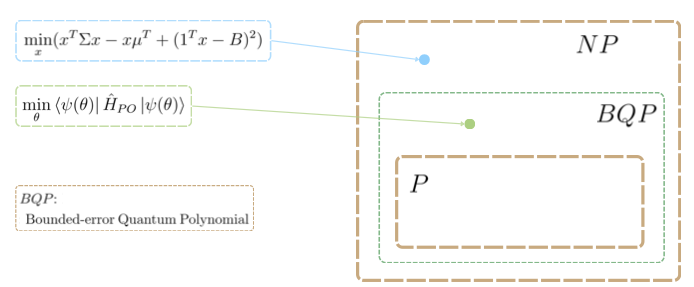
\includegraphics[width=0.8\textwidth]{images/complessita.png}
    \caption{Gerarchia delle classi di complessità computazionale.}
\end{figure}
\section{Algoritmi esistenti (QUBU)}\label{sec:algoritmi}

\subsection{VQA}\label{sec:vqa}




\subsection{Variational Quantum Eigensolver}\label{sec:vqe}

Il Variational Quantum Eigensolver (VQE) è un algoritmo ibrido che combina l'uso di 
computer quantistici e classici per risolvere problemi di ottimizzazione. Il suo 
funzionamento si basa sul principio variazionale e mira a trovare lo stato di energia 
minima di un sistema quantistico.

L'idea principale è quella di parametrizzare un circuito quantistico attraverso un 
insieme di parametri $\theta$ e utilizzare questi parametri per minimizzare l'energia 
del sistema, definita come:

\begin{equation}\label{eqn:energiaSistema}
    E(\theta) = \frac{
                    \langle\psi(\theta)|H|\psi(\theta)\rangle
                }
                {
                    \langle\psi(\theta)|\psi(\theta)\rangle
                },
\end{equation}

dove $H$ è l'Hamiltoniano che descrive il nostro problema di ottimizzazione e 
$\psi(\theta)$ è la funzione d'onda parametrizzata. In particolare, lo stato 
fondamentale $E_0$ corrisponde allo stato fondamentale (\textit{ground state}) 
di energia minima: 

\begin{equation}
    E_0 \le \frac{
                    \langle\psi(\theta)|H|\psi(\theta)\rangle
                }
                {
                    \langle\psi(\theta)|\psi(\theta)\rangle
                }.
\end{equation}

Quindi, il compito del VQE è trovare l'insieme ottimale di parametri, tale che 
l'energia associata allo stato sia quasi indistinguibile dal suo stato fondamentale, 
cioè trovare l'insieme di parametri $\theta$, corrispondente all'energia $E_{\min}$, 
per il quale $|E_{\min} - E_0| < \epsilon$, dove $\epsilon$ è una costante 
arbitrariamente piccola. Questo problema può essere formulato su un computer 
quantistico come una serie di gates, che vengono applicate allo stato iniziale 
per realizzare un ansatz strutturato per il problema Hamiltoniano. 

Convenzionalmente, lo stato iniziale è impostato per essere lo stato di vuoto, i.e., 
per un sistema di $N$ qubit $|0\rangle^{\otimes N} = |0\rangle$. 
Quindi, il problema di minimizzare l'energia del sistema (Equazione~\ref{eqn:energiaSistema}) 
può essere espresso come:

\begin{equation}
    E_{\min} = \min_{\theta} \langle 0|U^{\dagger}(\theta)HU(\theta)|0\rangle,
\end{equation}

dove $U(\theta)$ è l'operatore unitario parametrizzato che fornisce la funzione 
d'onda ansatz quando applicato allo stato iniziale, e $E_{\min}$ è l'energia 
associata all'ansatz parametrizzato.

Per essere efficientemente implementato in un circuito quantistico, è importante
che $H$ venga espresso nella forma:

\begin{equation}
    H = \sum_{l} c_l P_l = \sum_{l} c_l \otimes \sigma_j^i,
\end{equation}

dove \(P_l\) sono stringhe di Pauli rappresentate dal prodotto tensore degli 
operatori di Pauli \(\sigma_j^i \in \{I, \sigma_X, \sigma_Y, \sigma_Z\}\), 
con \(j\) che denota il qubit su cui l'operatore agisce e \(i\) il termine 
dell'Hamiltoniano. I coefficienti \(c_l\) sono pesi reali o complessi, 
adeguati per definire l'Hamiltoniano specifico del problema. In questa 
rappresentazione, l'Hamiltoniano è espresso come una combinazione lineare 
di stringhe di Pauli.

Quindi, l'obiettivo del VQE è risolvere il seguente problema di ottimizzazione:

\begin{equation}
    E_{\text{min}} = \min_\theta \sum_{l} c_l \langle 0 | U^\dagger(\theta) P_l U(\theta) | 0 \rangle.
\end{equation}

In questo contesto, si cerca lo stato \(|\psi(\theta)\rangle\) che corrisponde 
allo stato fondamentale di \(H\).

Il calcolo del valore atteso di una stringa di Pauli \(P_l\) è essenziale. 
Questo valore è ottenuto misurando ogni qubit coinvolto nella stringa \(P_l\), 
operando nella base di misura adeguata. Ad esempio, per uno stato generico del 
tipo \(|\psi\rangle = \alpha |0\rangle + \beta |1\rangle\), il valore atteso 
sull'operatore di Pauli \(\sigma_Z\) è dato da:

\begin{equation}
    \langle \psi | \sigma_Z | \psi \rangle = |\alpha|^2 - |\beta|^2.
\end{equation}

Questo valore rappresenta la probabilità di osservare lo stato \(|0\rangle\) meno 
la probabilità di osservare lo stato \(|1\rangle\). Misure relative a \(\sigma_X\) 
o \(\sigma_Y\) richiedono una rotazione preliminare nella base di misura \(\sigma_Z\).

Dato che i risultati delle misurazioni quantistiche sono binari, è necessario 
ripetere l'esperimento più volte per approssimare al meglio il valore medio 
di ogni termine. Questo processo è ripetuto separatamente per ogni stringa 
\(P_l\) che compone l'Hamiltoniano.

L'approccio VQE mira a bilanciare la complessità del circuito quantistico con il 
numero di misurazioni richieste, permettendo un'ottimizzazione efficiente degli 
stati parametrizzati. Il processo di ottimizzazione avviene in modo iterativo. 
Inizialmente, il computer quantistico prepara uno stato quantistico utilizzando 
i parametri correnti. Successivamente, viene misurata l'energia di questo stato 
preparato. Sulla base di questa misura, un ottimizzatore classico aggiorna i 
parametri nel tentativo di minimizzare l'energia del sistema. Questo ciclo di 
preparazione, misurazione e aggiornamento viene ripetuto fino a raggiungere la 
convergenza, ovvero fino a quando l'energia non può essere ulteriormente 
minimizzata in modo significativo.

Questo approccio ibrido sfrutta i punti di forza di entrambe le tipologie di 
computer: il computer quantistico si occupa della preparazione e della misurazione 
degli stati quantistici, mentre il computer classico gestisce l'ottimizzazione 
dei parametri. Nel contesto dell'ottimizzazione di portafoglio, il VQE viene 
impiegato per trovare la configurazione ottimale degli asset che minimizza una 
funzione obiettivo, tenendo conto sia del rischio che del rendimento atteso.

\begin{figure}[h!]
    \centering
    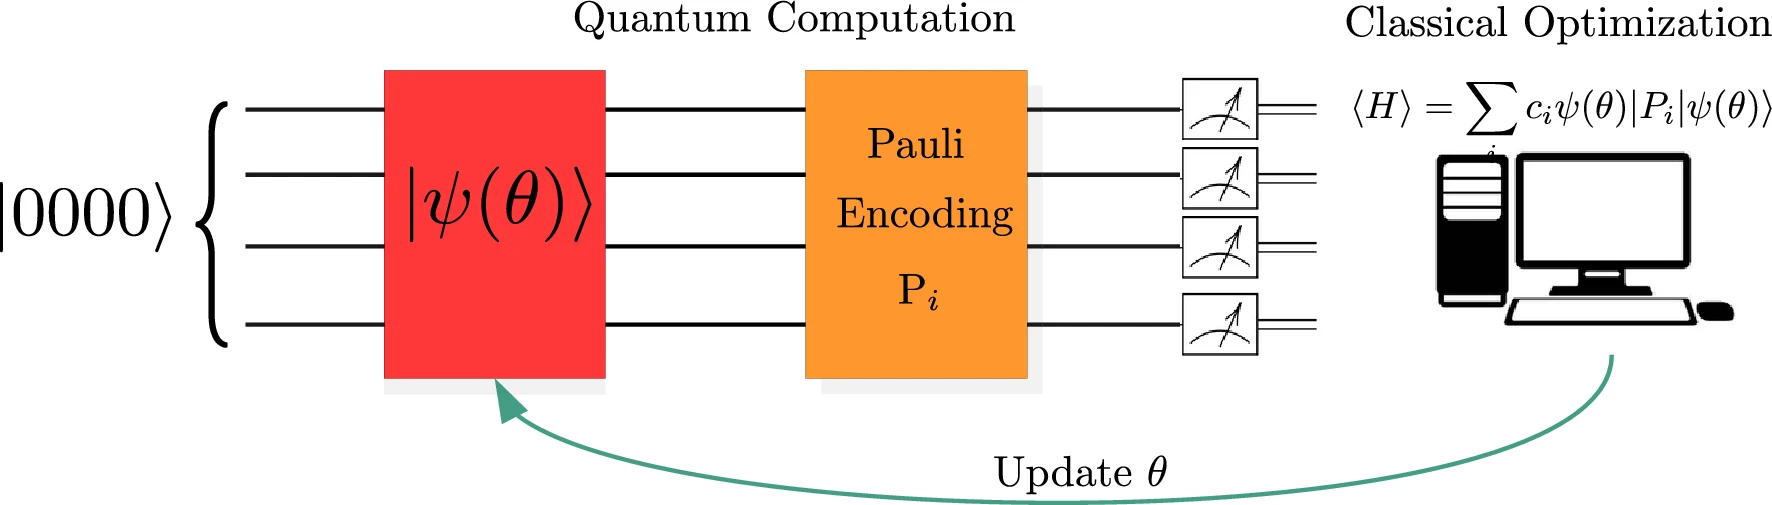
\includegraphics[width=0.9\textwidth]{images/vqe.png}
    \caption{Schema del funzionamento del Variational Quantum Eigensolver~\cite{buonaiuto2023best}.}
\end{figure}


\subsection{QAOA}\label{sec:qaoa}

\section{Validazione della soluzione proposta}
\label{sec:expval}

\section{Risultati}\label{sec:results}

Per l'analisi dei risultati senza rumore (\textit{noiseless}), è stata utilizza
una configurazione con 
8 asset, un budget massimo pari a 5, una penalità impostata sul valore del budget, 
un rischio pari al 20\% e 50 ripetizioni per ciascun algoritmo. 
La Figura~\ref{fig:noiseless-risultati-1} mostra rispettivamente la distribuzione 
delle selezioni effettuate dagli algoritmi QAOA, VQE e Exact Eigensolver.

\begin{figure}[ht!]
    \centering
    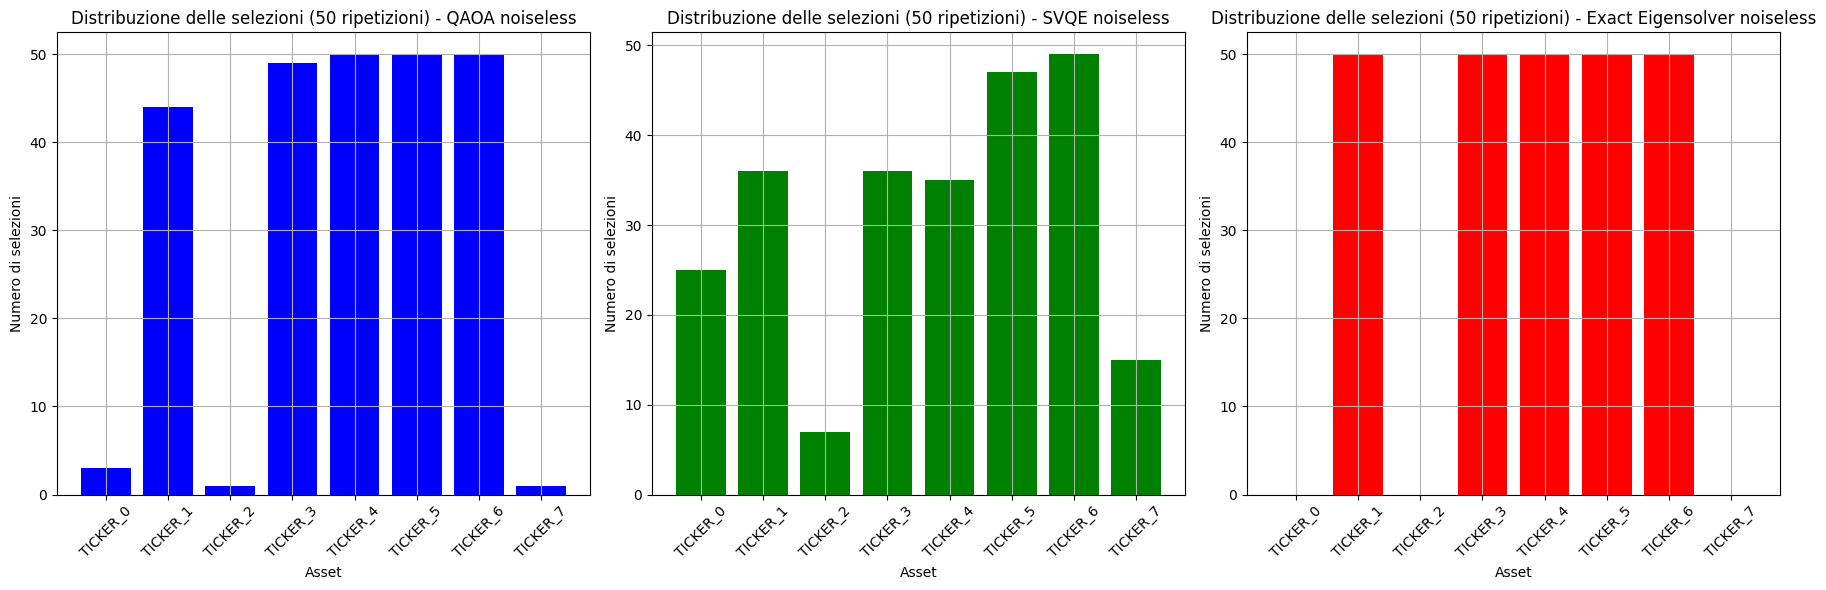
\includegraphics[width=0.99\textwidth]{images/risultati/noiseless-risultati-1.png}
    \caption{Distribuzione delle selezioni effettuate dagli algoritmi QAOA, VQE e Exact Eigensolver.}
    \label{fig:noiseless-risultati-1}
\end{figure}

L'algoritmo QAOA evidenzia una preferenza marcata per specifici asset, che vengono 
selezionati con una frequenza significativamente maggiore rispetto agli altri. 
Questo comportamento è legato alla natura parametrizzata dell'algoritmo e alla 
sensibilità verso i valori iniziali dei parametri scelti per l'ottimizzazione. 
Tuttavia, questa limitata capacità esplorativa può risultare in una perdita di 
soluzioni ottimali o in una convergenza verso configurazioni subottimali.

D'altra parte, il VQE mostra una distribuzione più variegata delle selezioni. 
La capacità dell'algoritmo di adattare i parametri dell'ansatz consente di 
esplorare con maggiore efficacia lo spazio delle soluzioni. Nonostante questa 
maggiore diversificazione, i risultati non sono sempre allineati con quelli 
ottimali, evidenziando che alcune incertezze permangono anche in questo caso.

L'Exact Eigensolver rappresenta la \textit{ground truth} del problema. Questo 
metodo fornisce sempre la soluzione esatta e ottimale del problema, servendo 
da riferimento principale per valutare la qualità dei risultati ottenuti con 
gli approcci approssimati.

La Figura~\ref{fig:noiseless-risultati-2} confronta le distribuzioni delle 
selezioni dei tre algoritmi, evidenziando le principali differenze. Il QAOA 
tende a concentrare le sue scelte su un insieme ristretto di asset, 
confermando una minore capacità esplorativa rispetto al VQE, che riesce 
invece a bilanciare meglio esplorazione ed exploitazione.

Infine, la Figura~\ref{fig:noiseless-risultati-3} analizza la frequenza 
delle combinazioni di asset selezionate nelle 50 ripetizioni. Anche qui 
si nota come il QAOA presenti una concentrazione delle combinazioni 
selezionate, mentre il VQE esplora una maggiore varietà di configurazioni. 


\begin{figure}[ht!]
    \centering
    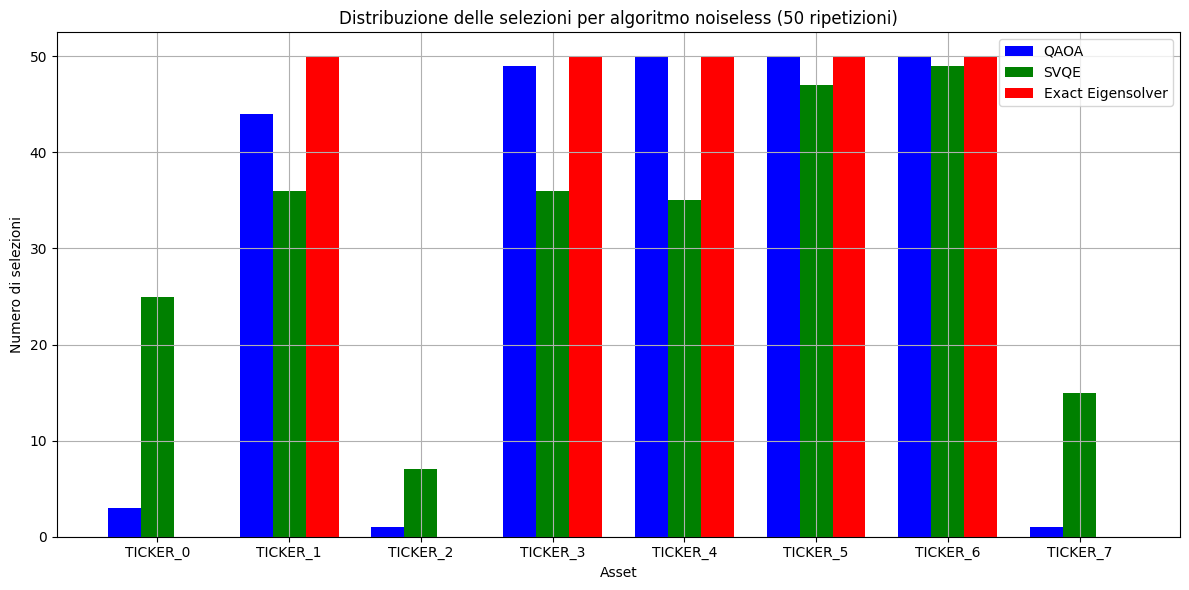
\includegraphics[width=0.99\textwidth]{images/risultati/noiseless-risultati-2.png}
    \caption{Distribuzione delle selezioni per algoritmo.}
    \label{fig:noiseless-risultati-2}
\end{figure}
\begin{figure}[ht!]
    \centering
    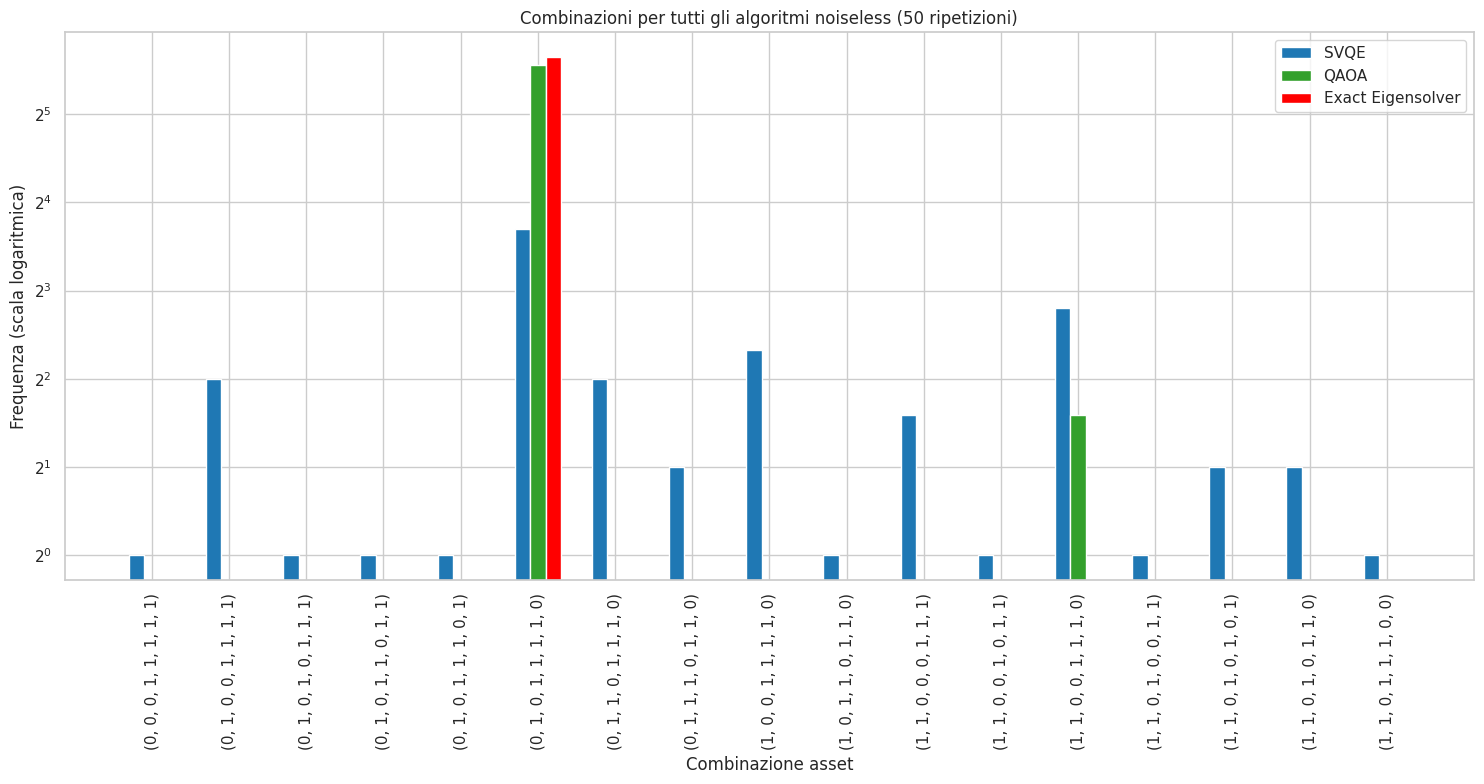
\includegraphics[width=0.99\textwidth]{images/risultati/noiseless-risultati-3.png}
    \caption{Frequenza delle combinazioni di asset selezionate nei 50 esperimenti.}
    \label{fig:noiseless-risultati-3}
\end{figure}


\subsection{Risultati con l'introduzione del rumore}

Per l'analisi dei risultati condizionati dal rumore (\textit{noisy}), 
è stata utilizzata la stessa configurazione 
di base con 8 asset, un budget massimo pari a 5, una penalità impostata sul valore 
del budget, un rischio pari al 20\% e 50 ripetizioni per ciascun algoritmo. 
La Figura~\ref{fig:noisy-risultati-1} mostra rispettivamente la distribuzione 
delle selezioni effettuate dagli algoritmi QAOA e VQE in presenza di rumore.

\begin{figure}[ht!]
    \centering
    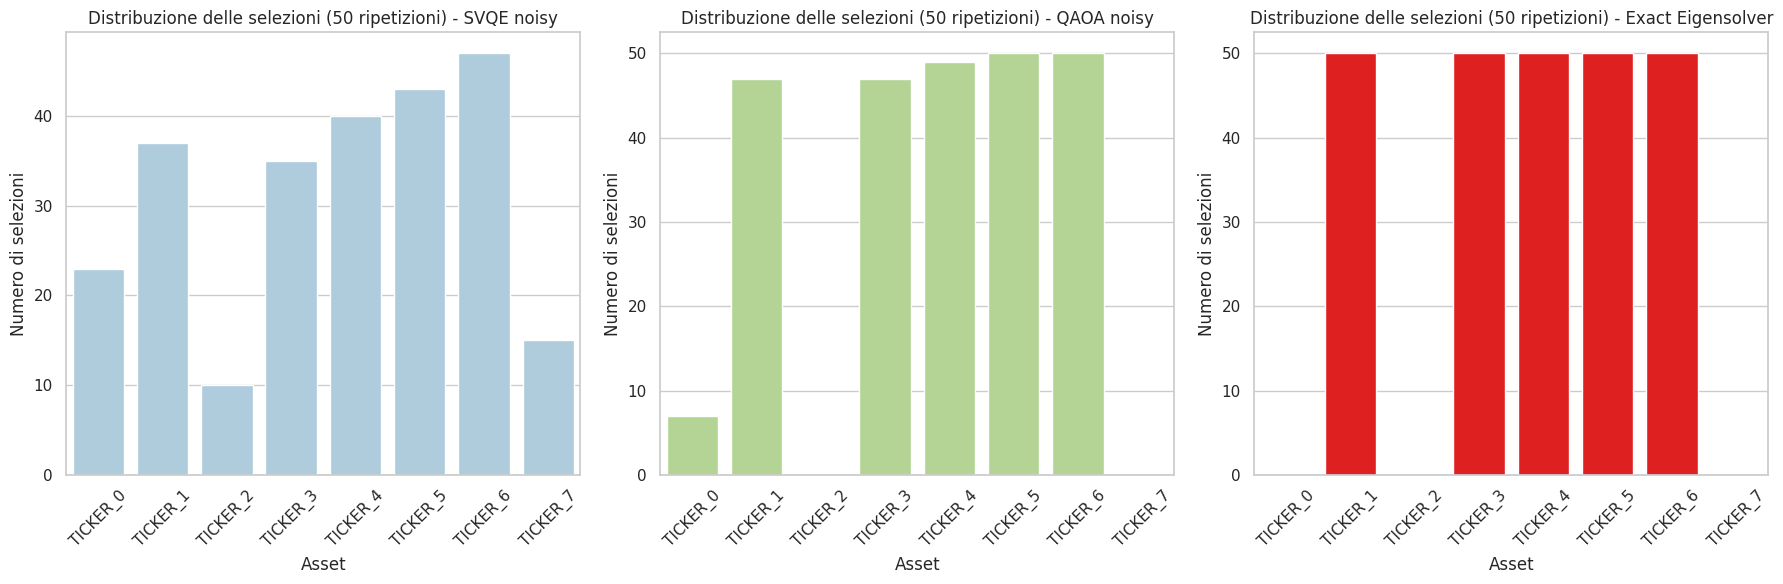
\includegraphics[width=0.99\textwidth]{images/risultati/noisy-risultati-1.png}
    \caption{Distribuzione delle selezioni effettuate dagli algoritmi QAOA e VQE in presenza di rumore.}
    \label{fig:noisy-risultati-1}
\end{figure}

L'algoritmo QAOA, in presenza di rumore, mostra una distribuzione delle selezioni 
meno concentrata rispetto alla versione noiseless. Questo comportamento 
è dovuto alla sensibilità dell'algoritmo ai rumori di decoerenza e di gate, 
che influenzano negativamente la capacità di esplorare al meglio lo spazio 
delle soluzioni. 

Il VQE, sebbene anch'esso influenzato dal rumore, riesce a mantenere una 
distribuzione delle selezioni più variegata rispetto al QAOA. La capacità 
dell'algoritmo di adattare i parametri dell'ansatz consente di mitigare 
parzialmente gli effetti del rumore, sebbene i risultati mostrino comunque 
una riduzione della qualità delle soluzioni rispetto alla versione noiseless.

La Figura~\ref{fig:noisy-risultati-2} confronta le distribuzioni delle selezioni 
dei due algoritmi in presenza di rumore, evidenziando le principali differenze. 

Infine, la Figura~\ref{fig:noisy-risultati-3} analizza la frequenza delle combinazioni 
di asset selezionate nelle 50 ripetizioni in presenza di rumore.

\begin{figure}[ht!]
    \centering
    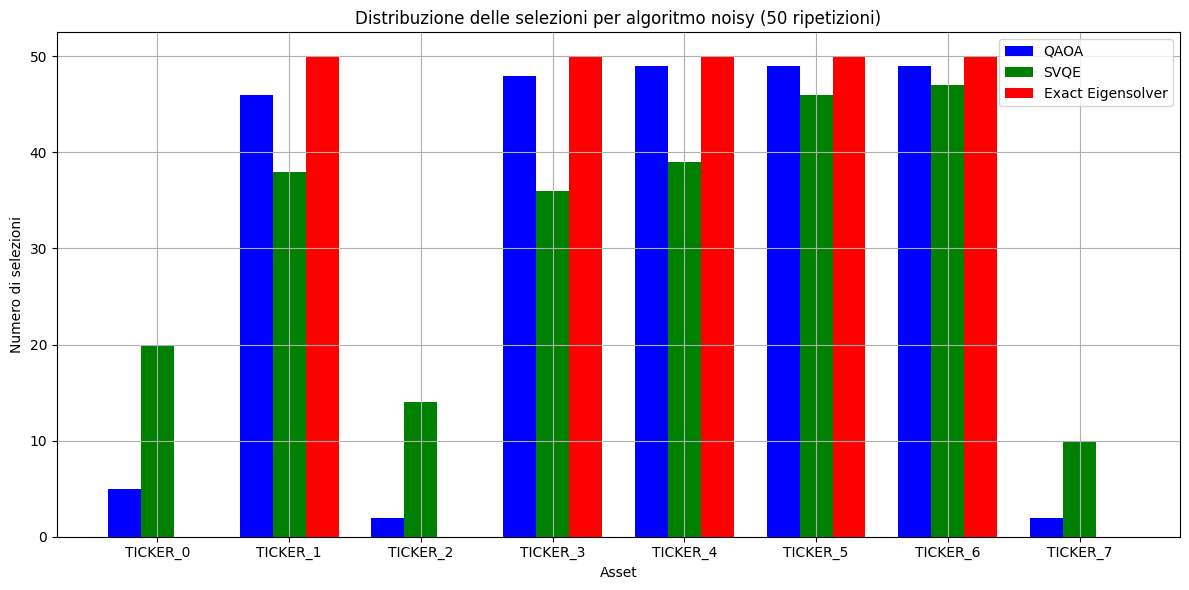
\includegraphics[width=0.99\textwidth]{images/risultati/noisy-risultati-2.png}
    \caption{Distribuzione delle selezioni per algoritmo in presenza di rumore.}
    \label{fig:noisy-risultati-2}
\end{figure}
\begin{figure}[ht!]
    \centering
    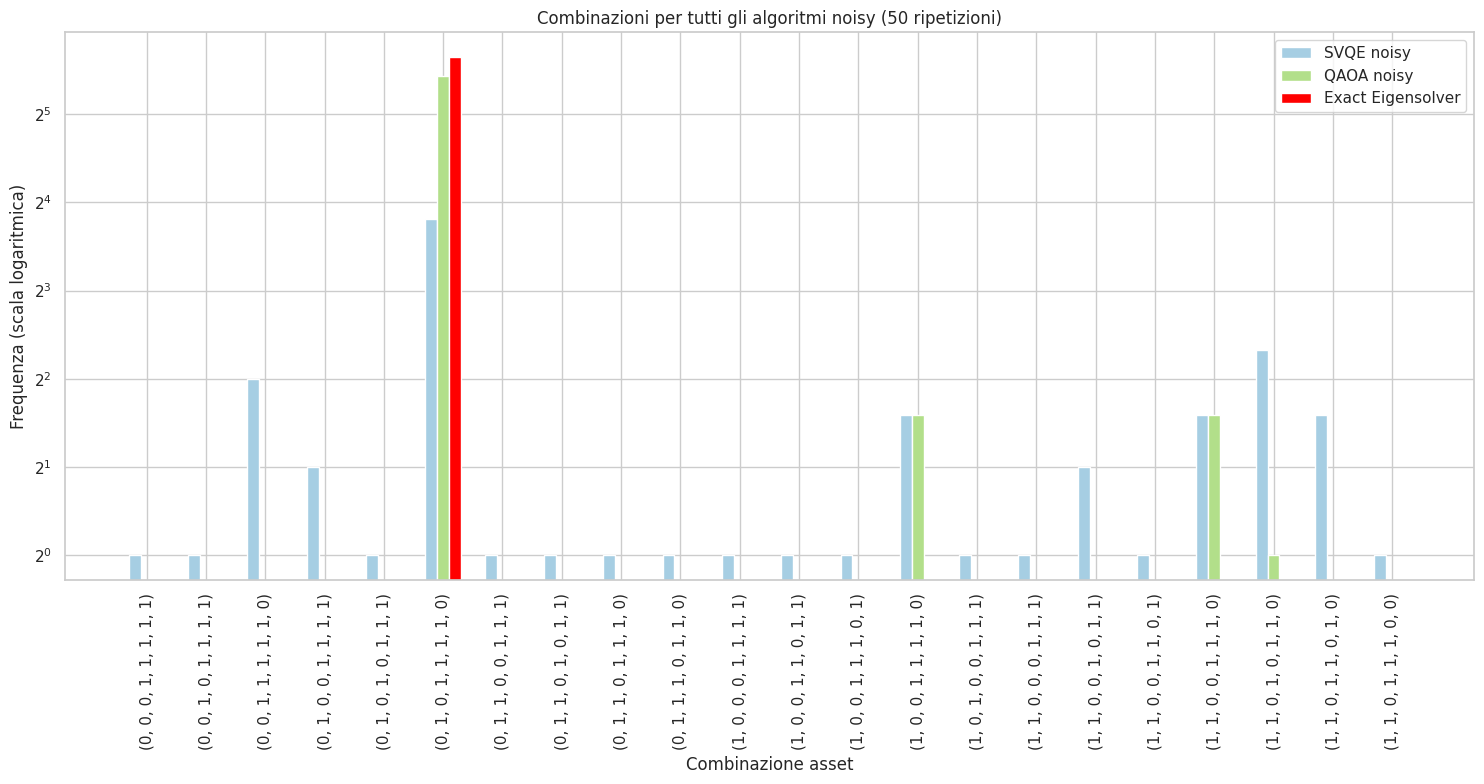
\includegraphics[width=0.99\textwidth]{images/risultati/noisy-risultati-3.png}
    \caption{Frequenza delle combinazioni di asset selezionate nei 50 esperimenti in presenza di rumore.}
    \label{fig:noisy-risultati-3}
\end{figure}


\paragraph{Confronto algoritmi (noiseless vs noisy)}
Quest'ultimo confronto ci permette di valutare l'impatto 
del rumore sulle prestazioni degli algoritmi e sulla qualità delle soluzioni ottenute.

La Figura~\ref{fig:confronto-svqe-noiseless-noisy} mostra il confronto delle combinazioni selezionate 
dall'algoritmo VQE in condizioni noiseless e noisy. Si può osservare che, in presenza 
di rumore, l'algoritmo VQE tende a selezionare un insieme più variegato di combinazioni 
rispetto alla versione noiseless. Questo comportamento è dovuto alla capacità 
dell'algoritmo di adattare i parametri dell'ansatz, che consente di esplorare con 
maggiore efficacia lo spazio delle soluzioni anche in presenza di rumore. Tuttavia, 
la qualità complessiva delle soluzioni ottenute dal VQE risulta inferiore rispetto a 
quella del QAOA, evidenziando una maggiore difficoltà nell'ottenere una scelta ottimale 
delle soluzioni in presenza di rumore.

La Figura~\ref{fig:confronto-qaoa-noiseless-noisy} mostra il confronto delle combinazioni selezionate 
dall'algoritmo QAOA in condizioni noiseless e noisy. Anche in questo caso, si nota un 
insieme più variegato di soluzioni in presenza di rumore, ma comunque non ci si 
allontana di molto dalla soluzione ottimale. L'algoritmo QAOA, nonostante la presenza 
di rumore, riesce a mantenere una buona qualità delle soluzioni, dimostrando una 
maggiore robustezza rispetto al VQE.

\begin{figure}[ht!]
    \centering
    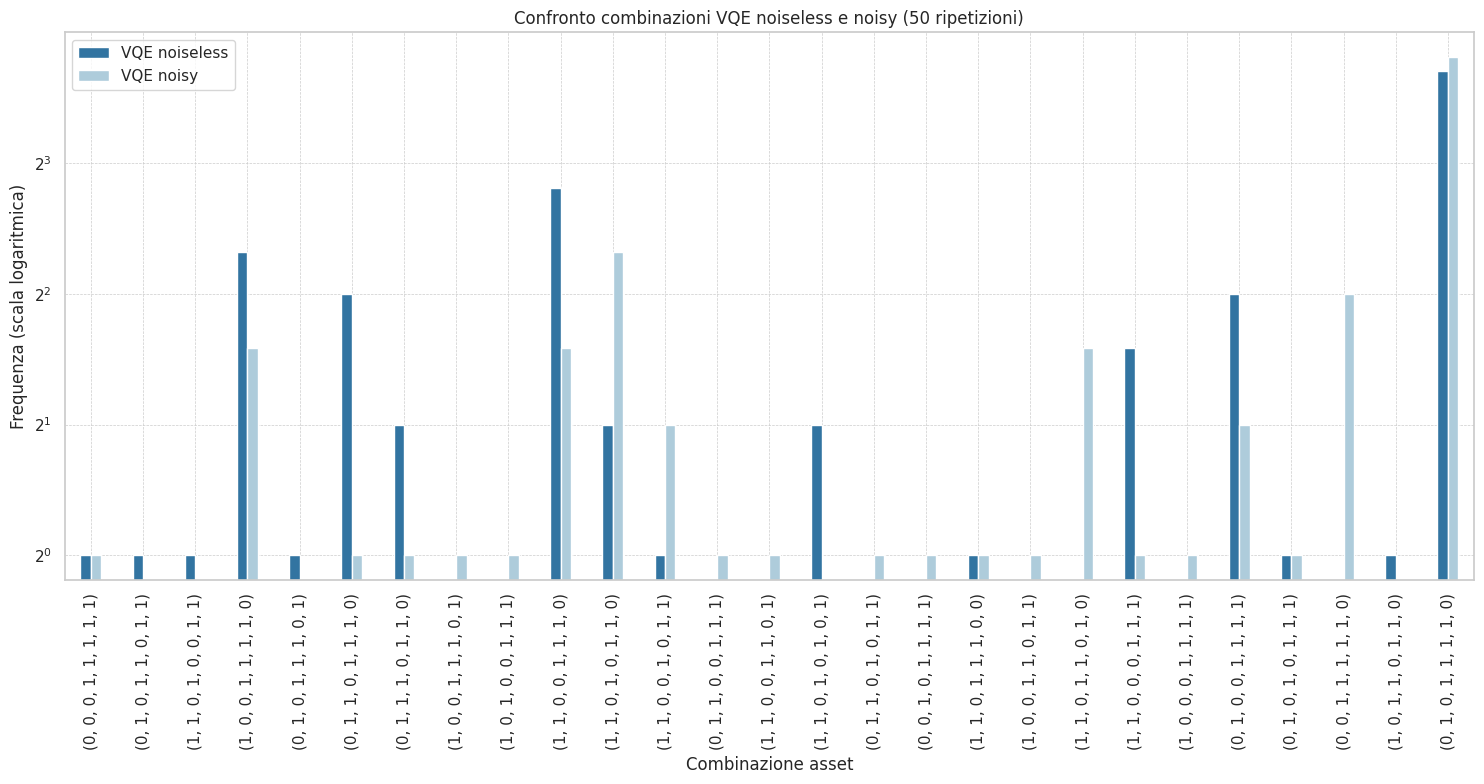
\includegraphics[width=0.99\textwidth]{images/risultati/confronto-svqe.png}
    \caption{Confronto delle combinazioni selezionate dall'algoritmo VQE in condizioni noiseless e noisy.}
    \label{fig:confronto-svqe-noiseless-noisy}
\end{figure}

\begin{figure}[ht!]
    \centering
    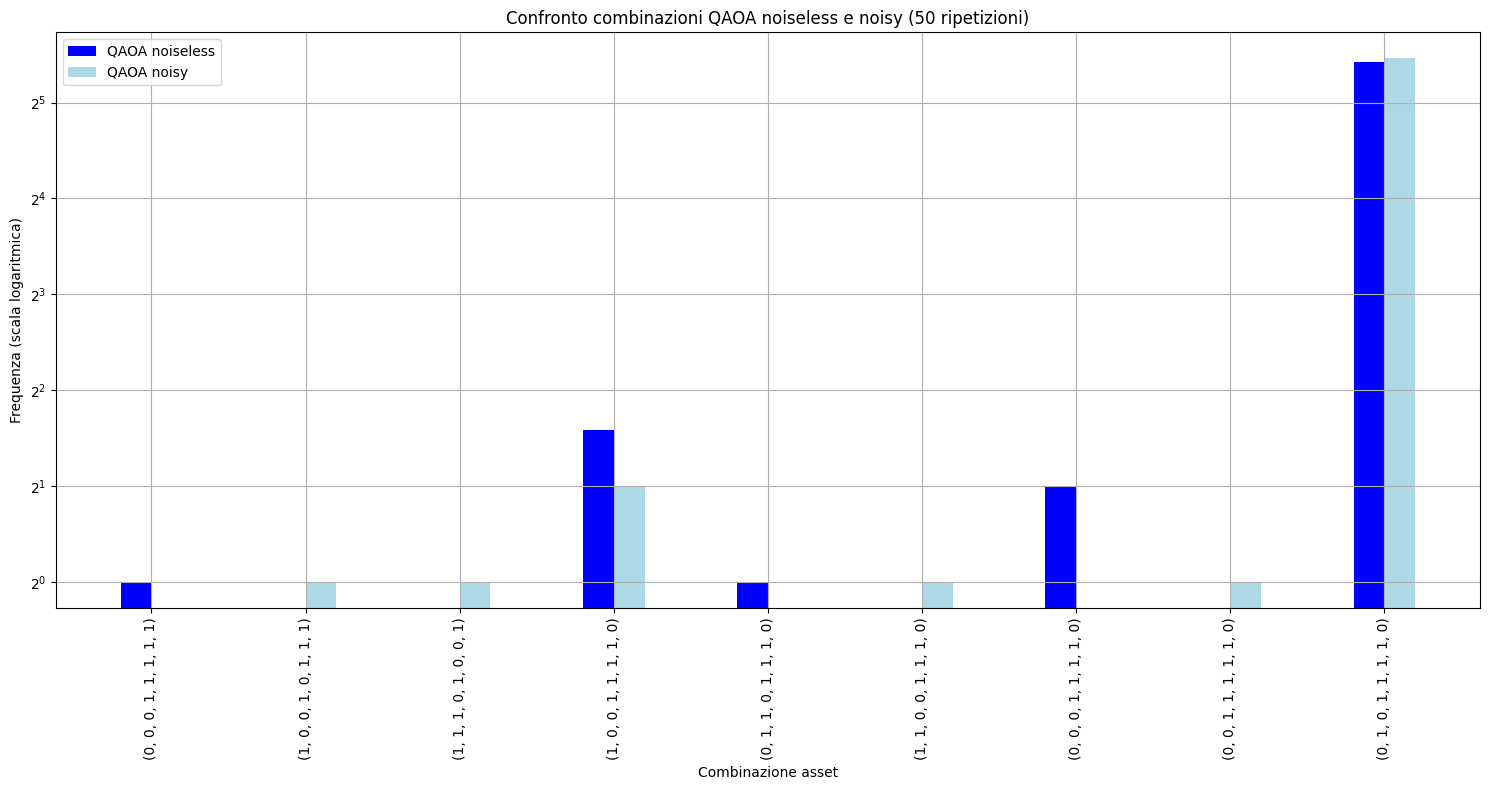
\includegraphics[width=0.99\textwidth]{images/risultati/confronto-qaoa.png}
    \caption{Confronto delle combinazioni selezionate dall'algoritmo QAOA in condizioni noiseless e noisy.}
    \label{fig:confronto-qaoa-noiseless-noisy}
\end{figure}



\section{Conclusioni}
\label{sec:conclusion}


\textit{Acknowledgments} \\ 
Questo progetto è stato realizzato durante il corso di Quantum Computing 
(a.a. 2024--25), presso l'Università degli Studi di Parma. \\
Il codice sorgente è disponibile su Github: 
\begin{center}
  \url{https://github.com/merendamattia/quantum-portfolio-optimization}.
\end{center}

\hfill

\break
\printbibliography

\end{document}
